\chapter{Аналитический раздел}

В данном разделе представлены базовые сведения о графовых структурах, обоснован выбор используемой графовой структуры и описано техническое задание.

\section{Техническое задание}

Задана система двусторонних дорог.
Определить, можно ли, построив еще три новые
дороги, из заданного города добраться до
каждого из остальных городов, проезжая
расстояние не более Т единиц.

\section{Теоритические сведения}

Граф – это конечное множество вершин и ребер, соединяющих их:

\begin{equation}
    G = < V, E >,
\end{equation}

где $V$ – конечное непустое множество вершин; $E$ – множество ребер (пар
вершин).

Если пары $E$ (ребра) имеют направление, то граф называется ориентированным
(орграф), если иначе - неориентированный (неорграф). Если в пары $E$ входят только
различные вершины, то в графе нет петель. Если ребро графа имеет вес, то граф
называется взвешенным. Степень вершины графа равна числу ребер, входящих и
выходящих из нее (инцидентных ей). Неорграф называется связным, если существует
путь из каждой вершины в любую другую.

\section{Представление графа в памяти}

\subsection{Матрица смежностей}

Графы в памяти могут представляться различным способом. Один из видов
представления графов – это матрица смежности $B(n\times n)$; В этой матрице элемент
$b[i,j] = 1$, если ребро, связывающее вершины $V_i$ и $V_j$ существует и $b[i,j] = 0$, если ребра
нет. У неориентированных графов матрица смежности всегда симметрична.

\subsection{Список смежностей}

Во многих случаях удобнее представлять граф в виде так называемого списка
смежностей. Список смежностей содержит для каждой вершины из множества
вершин $V$ список тех вершин, которые непосредственно связаны с этой вершиной.
Каждый элемент ($ZAP[u]$) списка смежностей является записью, содержащей данную
вершину и указатель на следующую запись в списке (для последней записи в списке
этот указатель – пустой). Входы в списки смежностей для каждой вершины графа
хранятся в таблице (массиве) ($BEG [u]$)

\subsection{Вывод}

Для решения поставленной задачи было решено хранить матрицу в виде матрицы смежности, так как работа осуществляется с взвешенным неориентированным графом. Ребер в рассматриваемых графах достаточно много, так что реализация списком не будет выигрывать по памяти.

\section{Алгоритмы поиска кратчайшего пути}

\subsection{Алгоритм Дейкстры}

Поиск кратчайших путей до всех вершин из одной указанной вершины для
взвешенного орграфа (имеющего значение, т.е. вес или стоимость, ребра) с
неотрицательными ребрами осуществляется с использованием алгоритма Дейкстры.
Алгоритм Дейкстры основан на выборе для включения в путь всякий раз той
вершины, которая имеет наименьшую оценку кратчайшего пути (по весам ребер), то
есть наименьший путь до этой вершины из всех возможных путей.

\subsection{Алгоритм Беллмана-Форда}

Алгоритм Беллмана-Форда позволяет решить задачу о поиске кратчайших
путях из одной выбранной вершины ко всем остальным вершинам при любых весах
ребер, в том числе и отрицательных. Сначала ищется путь от выбранной вершины ко
всем вершинам, связными с ней (аналогично поиску в ширину), а затем – кратчайший
путь ко всем остальным вершинам, с попыткой последовательно пройти к ним, т.е.
сначала через первую вершину, затем через вторую, через третью и так далее до
последней вершины. Кроме того алгоритм возвращает TRUE, если в графе нет цикла
отрицательного веса, достижимого из данной вершины.

\subsection{Алгоритм Флойда-Уоршалла}

Для поиска кратчайших путей между всеми вершинами используется алгоритм
Флойда-Уоршалла. По алгоритму Флойда-Уоршалла сначала ищется кратчайший
путь от одной вершины ко всем вершинам, доступным из нее, затем проводятся те же
действия, но пытаясь пройти от этой вершины ко всем доступным из нее, проходя
каждый раз через новую вершину (сначала через первую, затем – через вторую и
т.д.). Таким образом обрабатываются все вершины.

\subsection{Вывод}

Для решения реализуемым программным обеспечением поставленной задачи необходимо использовать алгоритм Дейкстры, так как осуществляется поиск кратчайших путей до всех вершин из данной, а также веса графов положительные.

\chapter{Конструкторский раздел}

В данном разделе описаны используемые структуры данных, приведен листинг используемых функций, а также описан алгоритм Дейкстры.

\section{Структуры данных}

Используемые структуры данных представлены ниже, на листинге \ref{lst:structs}

\begin{lstlisting}[language=C,caption=Используемые структуры данных,label=lst:structs]
// Структура очереди

typedef struct node
{
    int key;
    struct node *next;
} node_t;


typedef struct
{
    node_t *first;
    node_t *last;
} queue_t;

// Структура графа

typedef struct graph
{
    unsigned int size;
    int **adjmat;
} graph_t;

\end{lstlisting}

\section{Используемые функции}

Ниже, на листинге \ref{func:queue}, представлены функции для работы с очередью.

\begin{lstlisting}[language=C,caption=Функции для работы с очередью,label=func:queue]
queue_t queue_empty(void);

void queue_push(queue_t *queue, int key);

int queue_pop(queue_t *queue);

void queue_destroy(queue_t *queue);
\end{lstlisting}

Ниже, на листинге \ref{func:graph}, представлены функции для работы с графом.

\begin{lstlisting}[language=C,caption=Функции для работы с графом,label=func:graph]
graph_t graph_init(unsigned int vertices);

void graph_output(const graph_t *graph, const char *graphname);

void graph_free(graph_t *graph);

int graph_input(graph_t *graph, const char *filename);

void graph_output(const graph_t *graph, const char *out);

void debug_out(const graph_t *graph);

bool graph_reachable(const graph_t *graph, int T, int src);
\end{lstlisting}

\section{Схемы алгоритмов}

Ниже, на рисунке \ref{algo}, представлена схема алгоритма Дейкстры.

\begin{figure}[h]
    \centering
    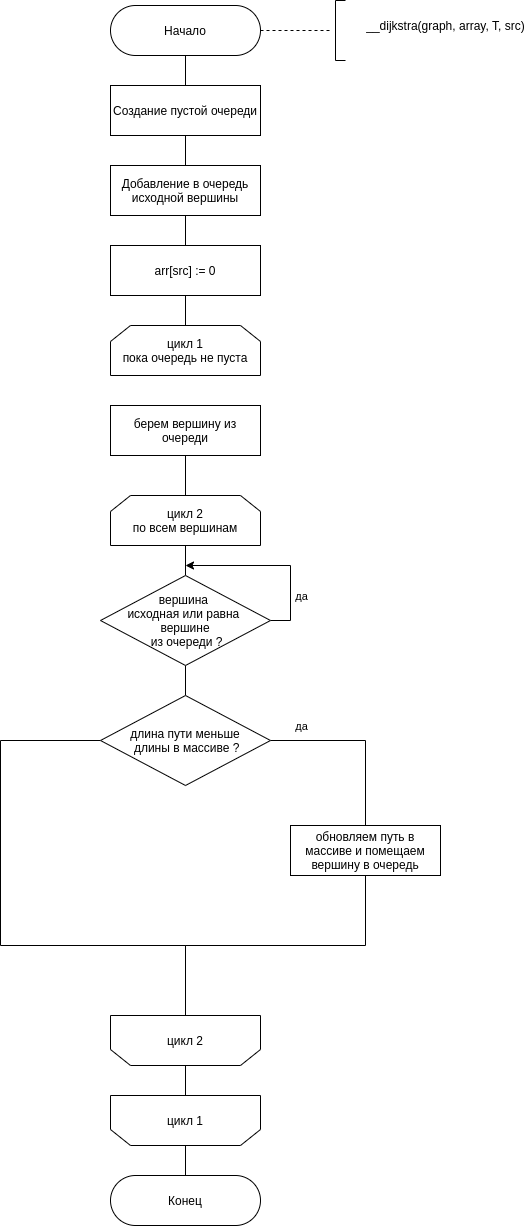
\includegraphics[width=0.6\linewidth]{dijkstra.png}
    \caption{Алгоритм Дейкстры}
    \label{algo}
\end{figure}

\chapter{Технологический раздел}

В данном разделе представлены предъявляемые к ПО требования, а также приведены функциональные тесты к разработанному ПО.

\section{Требования к ПО}

К разрабатываемому ПО предъявлены следующие требования:

\begin{itemize}[$\bullet$]
    \item На вход программе подается имя текстового файла, содержащего размер графа и всевозможные связи, а также максимальная длина пути и длины достраиваемых дорог.
    \item На выход программа синтезирует графическое представление введенного графа, а также графа с достроенными дорогами и результат: возможно ли добраться до каждой вершины из исходной за T.
\end{itemize}

\section{Тестирование ПО}

Ниже, на таблице \ref{table}, представлены функциональные тесты к разрабатываемому ПО.

\begin{table}
    \begin{center}
        \caption{Функциональные тесты}
        \begin{tabular}{|c|c|c|}
            \hline
            Входные данные & Выходные данные & Ожидаемый результат \\
            \hline
            \specialcell{Пустой файл} & 5 graph.txt & Incorrect input \\
            \hline
            \specialcell{Некорректный файл} & 5 g.jpg & Incorrect input \\
            \hline
            \specialcell{Некорректный размер \\ графа} & 5 graph.txt & Incorrect input \\
            \hline
            \specialcell{Некорректные ребра \\ графа} & 5 Incorrect input & Incorrect input \\
            \hline
            \specialcell{Некорректные вершины \\ графа} & 5 graph.txt & Incorrect input \\
            \hline
            \specialcell{Некорректный максимальный \\ путь} & -10 & Incorrect input \\
            \hline
            \specialcell{Исходная вершина больше \\ размера графа} & 10 graph.txt 222 & Incorrect input \\
            \hline
            \specialcell{Обычный тест} & 10 graph.txt 0 & Reachable \\
            \hline
        \end{tabular}
        \label{table}
    \end{center}
\end{table}

Все тесты пройдены успешно. \cite{test}

\chapter{Контрольные вопросы}

\begin{enumerate}
    \item Что такое граф?
    
    Граф - это конечный набор вершин и соединяющих их рёбер. Если ребра имеют направление, то граф называется ориентированным.

    \item Как представляются графы в памяти?
    
    В зависимости от поставленной задачи графы могут представляться в виде списка вершин и матрицы смежности этих вершин, либо с помощью списков смежности. Выбор зависит от соотношения между количеством вершин и количеством дуг в графе.

    \item Какие операции возможны над графами?
    
    В графах можно производить поиск отдельных вершин или рёбер, находить кратчайшие расстояния между вершинами, определять компоненты связности графа, а также его ацикличность.

    \item Какие способы обхода графов существуют?
    
    Обход в глубину (DFS - Depth First Search). При таком обходе, начиная с произвольной вершины $v_0$ ищется ближайшая смежная вершина $v$, для которой, в свою очередь, осуществляется поиск в глубину (т.е. снова ищется ближайшая, смежная с ней вершина) до тех пор, пока не встретится ранее просмотренная вершина, или не закончится список смежности вершины $v$ (то есть вершина полностью обработана). Если нет новых вершин, смежных с $v$, то вершина $v$ считается использованной, идет возврат в вершину, из которой попали в вершину $v$, и процесс продолжается до тех пор, пока не получим $v = v_0$.

    Обход в ширину (BFS - Breadth First Search). Обработка вершины $v$ осуществляется путем просмотра сразу всех новых соседей этой вершины. При этом полученный путь является кратчайшим путем из одной вершины в другую.

    \item Где используются графовые структуры?
    
    Графовые структуры активно применяются для представления сетевых отношений в базах данных. Также распростанено их пременение в нейронных сетях.

    \item Какие пути в графе Вы знаете?
    
    Путь --- последовательность вершин графа, соедененных ребрами.
	Простой путь --- путь без повторения вершин.
	Цепь --- путь без повторения ребер.
	Простая цепь --- цепь без повторения вершин.	
	Цикл --- путь, начальная и конечная вершина которого совпадают.
	Простой цикл --- цикл, который не проходит дважды по одной вершине.
	Гамильтонов путь (цикл) --- простая цепь (простой цикл), содержащая(ий) все вершины графа без повторений.

    \item Что такое каркасы графа?
    
    Каркас графа (остовное дерево) --- связный подграф, содержащий все вершины графа и не имеющий циклов. Количество ребер в каркасе связного графа всегда на единицу меньше количества вершин графа.
\end{enumerate}


